\documentclass[preview]{standalone}

\usepackage{amsmath}
\usepackage{amssymb}
\usepackage{stellar}
\usepackage{bettelini}
\usepackage{definitions}
\usepackage{tkz-tab}
\usepackage{xfrac}

\begin{document}

\id{sequences-functions-exercises}
\genpage

\section{Exercises}

\begin{snippetexercise}{sequence-of-functions-ex1}{}
    Consider the \sequence of functions
    \[
        f_n(x) = \frac{nx}{1 + n^2x^2}
    \]
    \begin{enumerate}
        \item Show that it converges pointwise in \(\realnumbers\) and that is converges uniformly on \([1, +\infty)\).
        \item Show that it does not converge uniformly in \([0,1]\).
        \item For \(x\in [0,1]\) compute
        \[
            F_n(x) \triangleq \integral[0][x][f_n(y)][y], \quad n \in \naturalnumbers
        \]
        show that \(\{F_n\}_{n \in \naturalnumbers}\) converges uniformly on \([0,1]\).
    \end{enumerate}
\end{snippetexercise}

\begin{snippetsolution}{sequence-of-functions-ex1-sol}{}
    We start by noting that \(f_n(0) = 0\).
    Let \(x \neq 0\), then
    \[
        |f_n(x)| = \frac{n|x|}{1 + n^2x^2} \leq \frac{n|x|}{n^2x^2} = \frac{1}{n|x|} \to 0
    \]
    as \(n\to\infty\).
    Thus \(f_n(x)\) converge puntualmente a \(f\equiv 0\).
    Per la convergenza uniforme abbiamo
    \begin{align*}
        \sup_{x\in [1; \infty)} |f_n(x) - f(x)| &=
        \sup_{x\in [1; \infty)} \frac{n|x|}{1 + n^2x^2}
    \end{align*}
    Studiamo la derivata
    \begin{align*}
        f_n'(x) &= \frac{
            n(1 + n^2x^2) - nx(2n^2x)
        }{
            {(1 + n^2x^2)}^2
        } = \frac{
            n(1 - n^2x^2)
        }{
            (1 + n^2x^2)
        } = 0
    \end{align*}
    che ha segno
    \begin{center}
        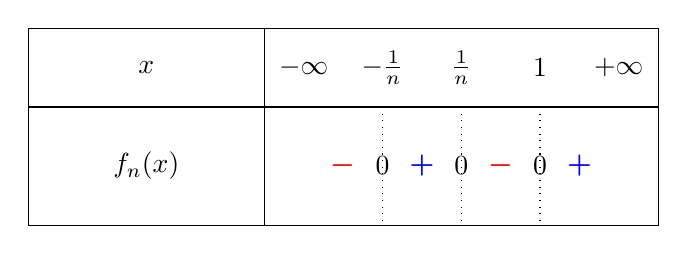
\begin{tikzpicture}
        % lgt = larghezza colonna sinistra, espcl = distanza tra i punti
        \tkzTabInit[lgt=3, espcl=1]
        {$x$ / 1, $f_n(x)$ / 1.5} % Etichette colonna sinistra / altezza riga
        {$-\infty$, $-\frac{1}{n}$, $\frac{1}{n}$, $1$, $+\infty$} % Punti critici

        % tkzTabLine inserisce i segni e gli zeri ("z" sta per zero)
        \tkzTabLine{
        , \textcolor{red}{\boldsymbol{-}}, 
        z, \textcolor{blue}{\boldsymbol{+}}, 
        z, \textcolor{red}{\boldsymbol{-}}, 
        z, \textcolor{blue}{\boldsymbol{+}}
        }
        \end{tikzpicture}
    \end{center}
    quindi visto che è sempre decrescente nell'insieme \([1, +\infty)\),
    il punto di massimo si ha in \(x=1\), cioè
    \[
        \sup_{x\in [1; \infty)} \frac{n|x|}{1 + n^2x^2}
        = f_n(0) = \frac{n}{1 + n^2} \to 0
    \]
    per \(n\to \infty\), quindi abbiamo convergenza uniforme.
    Nell'intervallo \([0,1]\), il punto di massimo è \(x = \sfrac1n\), quindi
    \[
        \sup_{x\in [0,1]} f_n(x) = f_n\left(\frac1n\right) = \frac12
    \]
    che non tende a \(0\) per \(n\to\infty\).
    Quindi non abbiamo continuità uniforme su \([0,1]\). Calcoliamo ora
    \begin{align*}
        F_n(x) = \integral[0][x][\frac{ny}{1 + n^2y^2}][y]
        = \frac{\log(1 + n^2x^2)}{2n}
    \end{align*}
    che tende a zero per \(n \to \infty\) per gerarchia degli infiniti, quindi converge puntualmente alla funzione nulla.
    Notiamo che siccome il logaritmo è una funzione monotona crescente, e pure \(1 + n^2x^2\) lo è per \(x>0\), allora tutta la funzione è
    monotona crescente, e quindi il suo massimo è in \(x=1\). Per la continuità uniforme abbiamo quindi
    \begin{align*}
        \sup_{x\in [0,1]} |F_n(x) - 0| &= f_n(1) = \frac{\log(1 + n^2)}{2n} \to 0
    \end{align*}
    per \(n\to\infty\), quindi abbiamo convergenza uniforme.
\end{snippetsolution}

\begin{snippetexercise}{sequence-of-functions-ex2}{}
    Study the uniform convergence of the \sequence of functions
    \[
        f_n(x) = \frac{n^2x^2}{1 + n^2x^2}
    \]
    and determine whether the following relation is true
    \[
        \lim_{n\to\infty} \integral[-1][1][f_n(x)][x] = \integral[-1][1][\lim_{n\to\infty}f_n(x)][x]
    \]
\end{snippetexercise}

\begin{snippetsolution}{sequence-of-functions-ex2-sol}{}
    Notiamo che \(f_n(0) = 0\). Se \(x\neq 0\); allora la funzione tende ad \(1\) per \(n\to\infty\). Abbiamo quindi convergenza puntuale
    \[
        f_n(x) \to f = \begin{cases}
            0 & x = 0 \\
            1 & x \neq 0
        \end{cases}
    \]
    Notiamo inoltre che \(f_n\) è continua, mentre \(f\) no su un dominio che contiene \(0\).
    Quindi, in un insieme che contiene \(0\), la funzione non converge uniformemente a \(f\).
    Studiamo se converge uniformemente ad \(f\) su un dominio della forma \(D=(-\infty, a) \union (b, +\infty)\) con \(a<0, b>0\).
    Abbiamo
    \begin{align*}
        \sup_{x\in D} |f_n - 1|
        &= \sup_{x\in D} \left|\frac{n^2x^2}{1+n^2x^2} - 1\right|
        =  \sup_{x\in D} \left|\frac{1}{1 + n^2x^2}\right|
        \leq \sup_{x\in D} \left|\frac{1}{1 + n^2C^2}\right| \to 0
    \end{align*}
    per \(n \to \infty\), dove abbiamo usato \(C = \min\{|a|, |b|\}\).
    Quindi abbiamo convergenza uniforme a \(f\) in \(D\), ma non su tutto \(\realnumbers\).
    Per la relazione abbiamo
    \begin{align*}
        \lim_n \integral[-1][1][f_n(x)][x]
        &= \lim_n \integral[-1][1][\frac{1 + n^2x^2}{1 + n^2x^2} - \frac{1}{1 + n^2x^2}][x]
        = \lim_n \left[x - \frac{\arctan(nx)}{n}\right]^1_1 \\
        &= \lim_n \left(
            1 - \frac{\arctan(n)}{n} + 1 - \frac{\arctan(n)}{n}
        \right) = \lim_n 2\left(
            1 - \frac{\arctan(n)}{n}
        \right) = 2
    \end{align*}
    e d'altra parte
    \[
        \integral[-1][1][\lim_n \frac{n^2x^2}{1 + n^2x^2}][x]
        = \integral[-1][1][1][x] = 2
    \]
    quindi la relazione vale.
\end{snippetsolution}

\begin{snippetexercise}{sequence-of-functions-ex3}{}
    Verify that the \sequence of function
    \[
        f_n(x) = x-\frac{x^n}{n}
    \]
    is not differentiable term by term on \([0,1]\).
\end{snippetexercise}

\begin{snippetsolution}{sequence-of-functions-ex3-sol}{}
    La funzione \(f_n(x)\) converge puntualmente a \(x\) in \([0,1]\).
    Studiamo la convergenza uniforme
    \[
        \sup_{x \in [0,1]} |f_n(x) - x| = \sup_{x \in [0,1]}
        \frac{x^n}{n} = \frac1n \to 0
    \]
    per \(n\to\infty\). Quindi \(f_n\) converge uniformemente a \(x\) su \([0,1]\).
    Da una parte abbiamo la derivata \((x)' = 1\), mentre dall'altra i termini della derivata
    \[
        f_n'(x) = 1- x^{n-1}
    \]
    che converge puntualmente a 
    \[
        f_n'(x) \to \begin{cases}
            1 & x \in [0,1) \\
            0 & x = 1
        \end{cases}
    \]
    che tuttavia non coincide con l'altra derivata in \(x=1\).
\end{snippetsolution}

\begin{snippetexercise}{sequence-of-functions-ex4}{}
    Consider the \sequence of functions
    \[ f_n(x) = \arctan(x^n) \]
    \begin{enumerate}
        \item Determine the \set of poinwise convergence \(S\) and the limit function \(f\).
        \item Verify that the \sequence does not converge uniformly on \(S\) and determine
        on which subintervals of \(S\) the \sequence converges uniformly. 
    \end{enumerate}
\end{snippetexercise}

\begin{snippetsolution}{sequence-of-functions-ex4-sol}{}
    We have the limit
    \[
        \lim_n \arctan(x^n) = \begin{cases}
            \nexists & x \leq -1 \\
            0 & x \in (-1,1) \\
            \frac\pi 4 & x = 1 \\
            \frac\pi 2 & x > 1
        \end{cases}
    \]
    so we have the pointwise convergence
    \[
        f_n(x) \to f = \begin{cases}
            0 & x \in (-1,1) \\
            \frac\pi 4 & x = 1 \\
            \frac\pi 2 & x>1
        \end{cases}
    \]
    on the \set \(S=(-1, \infty)\).
    Siccome le \(f_n\) sono continue e \(f\) è discontinua in \(x=1\), allora \(f_n\) non converge uniformemente ad \(f\)
    in \(S\). Studiamo la convergenza in \((1, \infty)\). Possiamo avvicinarci arbitrariamente a \(1^+\),
    e quindi
    \begin{align*}
        \sup_{x\in (1, +\infty)} \left|f_n(x) - \frac\pi 2\right| &=
        \sup_{x\in (1, +\infty)} \left|\arctan(x^n) - \frac\pi 2\right| \\
        &= \sup_{x\in (1, +\infty)} \left|\arctan(1) - \frac\pi 2\right| = \left|\frac\pi 4 - \frac\pi 2\right| > 0
    \end{align*}
    Quindi non vi è convergenza uniforme in un intorno di \(1\). Tuttavia, se \(a>1\),
    \[
        \sup_{x\in [a, +\infty)} \left|f_n(x) - \frac\pi 2\right|
        = \left|\arctan(a^n) - \frac\pi 2\right| \to 0
    \]
    per \(n\to\infty\), e quindi abbiamo convergenza uniforme su \([a,+\infty]\) con \(a>0\).
    Dalla parte sinistra con \(b<1\) per stare lontano da un intorno di \(x=1\), possiamo avvicinarci arbitrariamente a \(-1^+\), quindi
    \[
        \sup_{x \in (-1, b]} |f_n(x) - 0| =
        |\arctan({(-1)}^n)|
        = \frac\pi 2 > 0
    \]
    Tuttavia, sia \(-1<c<1\), abbiamo
    \[
        \sup_{x \in [c, b]} |f_n(x) - 0| =
        |\arctan(d^n)| \to 0
    \]
    per \(n\to\infty\), dove \(d = \max\{|b|, |b|\}\). Abbiamo quindi convergenza uniforme
    in \([c,b] \union [a,+\infty)\) per \(-1 < c < b < 1<a\).
\end{snippetsolution}

\begin{snippetexercise}{sequence-of-functions-ex5}{}
    Determine the limit function with respect to pointwise convergence on \(\realnumbers\) of the \sequence of functions
    \[
        f_n(x) = n\integral[
            x-\frac1n
        ][
            x+\frac1n
        ][e^{-t^2}][t]
    \]
    and prove that the convergence is uniform on \(\realnumbers\).
\end{snippetexercise}

\begin{snippetsolution}{sequence-of-functions-ex5-sol}{}
    \todo
\end{snippetsolution}

\begin{snippetexercise}{sequence-of-functions-ex6}{}
    Let \(f_n \colon \realnumbers^{\geq 0} \fromto \realnumbers\) and \(g_n \colon \realnumbers \fromto \realnumbers\) defined by
    \[
        f_n(x) \triangleq \sqrt{n^2 + nx}-n, \quad g_n(t) \triangleq \sqrt{
            \sin^2(t) + \frac1n
        }
    \]
    \begin{enumerate}
        \item Show that \(\{g_n\}\) converges uniformly on \(\realnumbers\) and that \(\{f_n\}\)
        converges uniformly on every bounded subset of \(\realnumbers^{\geq 0}\), but not on \(\realnumbers^{\geq 0}\). 
        \item Let \(\phi_n(t) = f_n(g_n(t))\). Show that \(\{\phi_n\}\) converges uniformly on \(\realnumbers\).
    \end{enumerate}
\end{snippetexercise}

\begin{snippetsolution}{sequence-of-functions-ex6-sol}{}
    \todo
\end{snippetsolution}

\begin{snippetexercise}{sequence-of-functions-ex7}{}
    Let \(f \colon [0, +\infty) \fromto \realnumbers\) of class \(\mathcal C^1\), for every \(n \in \naturalnumbers\) we define
    \(\varphi \colon [0, +\infty) \fromto \realnumbers\) such that
    \[
        \varphi_n(x) \triangleq \integral[0][x][f(t)\cos(nt)][t]
    \]
    Show that the \sequence \(\{\varphi(n)\}_{n \in \naturalnumbers}\) converges uniformly on \([0,b]\) for every \(b>0\). \\
    \emph{Hint:} use integration by parts.
\end{snippetexercise}

\begin{snippetsolution}{sequence-of-functions-ex7-sol}{}
    \todo
\end{snippetsolution}

\begin{snippetexercise}{sequence-of-functions-ex8}{}
    Consider the \sequence of functions \(\{f_n\}_{n\in\naturalnumbers}\) where, for every \(n \in \naturalnumbers\),
    \(f_n \colon [0,1] \fromto \realnumbers\) defined by
    \[ f_n(x) \triangleq n^2x^n(1-x) \]
    \begin{enumerate}
        \item Show that the \sequence converges pointwise on \([0,1]\).
        \item Show that the \sequence does not converge uniformly on \([0,1]\).
        \item Show that the \sequence converges uniformly on \([0,b]\), for every \(b \in (0,1)\).
        \item Determine whether the following equivalence holds:
        \[
            \lim_{n\to\infty} \integral[0][1][f_n(x)][x] = \integral[0][1][f(x)][x]
        \]
    \end{enumerate} 
\end{snippetexercise}

\begin{snippetsolution}{sequence-of-functions-ex8-sol}{}
    \todo
\end{snippetsolution}

\end{document}